\chapter{QT}
\section{Basics}
\begin{note}[QDebug header]\\
\verb|#include <QDebug>| and usage like \verb|qDebug() << "[" << this << "] m_size: " << m_size;|
\end{note}

\begin{note}[Signals and Slots]
\begin{enumerate}
\item In form designer, there is a signal/slot view (F4) which assist to define new signal/slots.
\item To add or remove s/s manually we can use \verb|connect| and \verb|disconnect|
\end{enumerate}
\begin{lstlisting} [language={c++}]
MainWindow::MainWindow(QWidget *parent) :
QMainWindow(parent), ui(new Ui::MainWindow)
{
  ui->setupUi(this);

  connect(ui->horizontalSlider,SIGNAL(valueChanged(int))
            ,ui->progressBar,SLOT(setValue(int)));
}
\end{lstlisting}
\end{note}

\begin{note}[Actions]
	
When you create a new menu, an action will be created, which can be drag and dropped on the toolbar. an actions allows u to trigger an event. rightclick $\rightarrow$ go to slots.
\end{note}

\begin{note}[setCentralWidget(object o)]
	
	You can use this function to set an object as the main widget on the form.
\end{note}

\begin{note}[Dialogs]
\begin{enumerate}
\item After creating a dialog, you need to include it the mainwindow.cpp (the parent window.) \verb|#include "mydialog.h"|
\item To show the dialog:
\verb|Dialog myDialog; myDialog->setModal(true); myDialog->exec();|
\item if u use exec, u cannot show the dialog modaless. we need to use show method for modaless dialogs, and also we should not define the dialog in stack, we need to define it on heap, so after the show function, the respected object wont be destroyed.
\begin{lstlisting} [language={c++}]
//In mainwindow.h
#include <dialog.h>
...
class MainWindow : public QMainWindow
{
   ...
private:
   Dialog *myDialog = nullptr;
};
//In mainwindow.cpp
void MainWindow::on_actionNew_Dialog_triggered()
{
   myDialog = new Dialog(this); //set this form as the parent
   myDialog->setModal(false);
   myDialog->show();
}
\end{lstlisting}
\end{enumerate}
\end{note}

\begin{note}[Minimal application with HTML aware widgets]
\begin{lstlisting}[language = {c++}]
#include <QApplication>
#include <QLabel>
int main(int argc, char *argv[])
{
   QApplication a(argc, argv);
   QLabel *l = new QLabel("<b>Hello</b> <font color=red><i>world");
   l->show();
   return a.exec();
}
\end{lstlisting}
\end{note}

\begin{note}[QHBoxLayout and QVBoxLayout]
\begin{enumerate}
	\item QHBoxLayout and QVBoxLayout are not widgets, so u cant show them unless u make a widget.
	\item There is a example below.
\end{enumerate}
\begin{lstlisting}[language = {c++}]
#include <QApplication>
#include <QLabel>
#include <QPushButton>
#include <QHBoxLayout>

int main(int argc, char *argv[])
{
  QApplication a(argc, argv);
  QLabel *l = new QLabel("<b>Hello</b> <font color=red><i>world");

  QWidget* window = new QWidget();
  QHBoxLayout* hlayout = new QHBoxLayout();

  hlayout->addWidget(new QPushButton("Hehe"));
  hlayout->addWidget(new QPushButton("HoHo"));
  hlayout->addWidget(new QPushButton("HerHer"));
  hlayout->addWidget(l);

  window->setLayout(hlayout);
  window->show();
  return a.exec();
}
\end{lstlisting}
\begin{center}
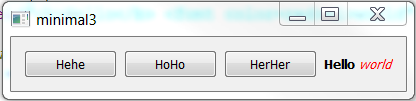
\includegraphics[]{Images/QT/HBox}
\end{center}
\end{note}

\begin{note}[QGridLayout]\\
Parameters in Order:\\
1.QWidget 2.Row Number 3.Column Number 4.Row Span 5.Column Span
\begin{lstlisting}[language = {c++}]
QGridLayout* main_layout = new QGridLayout(window);
main_layout->addWidget(new QPushButton("heheheh"),1,1,1,1);
main_layout->addWidget(new QPushButton("heheheh"),1,2,1,1);
main_layout->addWidget(new QPushButton("heheheh"),2,1,1,2);
\end{lstlisting}
\begin{center}
	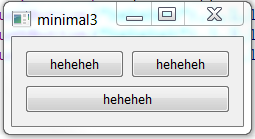
\includegraphics[]{Images/QT/QGrid}
\end{center}
\end{note}

\begin{note}[QSplitter]: u can add them by selection widgets in design view and click on the vertical/horizontal splitters
\end{note}

\begin{note}[QStatusBar]
\begin{lstlisting}[language = {c++}]
QLabel* lblStatusBar = new QLabel("Hi There");
...
ui->statusBar->addPermanentWidget(lblStatusBar);
ui->statusBar->showMessage("Hello",2000);
\end{lstlisting}
\end{note}

\begin{note}[QMessageBox]
\begin{lstlisting}[language = {c++}]
QString str[] = {"Hello","There"};
QMessageBox::critical(this,str[0],str[1],QMessageBox::YesAll);
\end{lstlisting}
\end{note}

\begin{note}[QTimer]
\begin{lstlisting}[language = {c++}]
QTimer* tmr = nullptr;

void main {
  tmr=new QTimer(this);
  tmr->setInterval(20);
  connect (tmr,SIGNAL(timeout()),this,SLOT(timerhit()));
  tmr->start();
}
//timerhit slot
void MainWindow::timerhit()
{
  ...
}
\end{lstlisting}
\end{note}

\begin{note}[Threads]
	
To build a thread, first we need to create a class that inherits from QThread and Q\_OBJECT should be emplaced in it.
\begin{lstlisting}[language = {c++}]
class Counter : public QThread
{
  Q_OBJECT
public:
  Counter();
};
\end{lstlisting}
Then we need to override the run() function. This is the thread entry. and also to provide bidirectional communication with the main thread, we need to define a signal, so it could be caught by the main thread if it was needed.
\begin{lstlisting}[language = {c++}]
class Counter : public QThread
{
  Q_OBJECT
private:
  bool blnStop = false;
public:
  Counter();
  void run() override;
signals:
  void NumberChanged (int);
};
void Counter::run() {
  static int i = 0;
  blnStop = false;
  while(!blnStop){
    //emit is used to raise the signal
    //it's equal to raise event in C#
    emit NumberChanged(++i);
    this->msleep(1);
  }
}
\end{lstlisting}
To find a way for stopping the thread from the outside, we can define a onQuit slot (or any other public function).
\begin{lstlisting}[language = {c++}]
public slots:
  void onQuit();
\end{lstlisting}
And finally to initialize and start it:
\begin{lstlisting}[language = {c++}]
void main ()
{
  c = new Counter();
  connect(c,SIGNAL(NumberChanged(int)),this,SLOT(onNumberChange(int)));
  c->start();
}
void MainWindow::onNumberChange(int i)
{
  ui->lblCount->setText(QString::number(i));
}
\end{lstlisting}
\end{note}
\begin{note}[QString]
\begin{itemize}
\item For converting numbers to QString
\begin{lstlisting}[language = {c++}]
Qstring str = QString::number(1);
\end{lstlisting}
\item For converting std::string to QString
\begin{lstlisting}[language = {c++}]
QString str = QString::fromStdString("AnSTDString");
\end{lstlisting}
\item For const char* to QString
\begin{lstlisting}[language = {c++}]
const char* psStr = "This is a string";
QString str(psStr);
\end{lstlisting}
\end{itemize}
\end{note}

\begin{note}[QList]
\begin{itemize}
\item It's like vector in std library;
\item Useful methods: append, removeat, removeOne, first, last, [], <<
\item it can be used in foreach loops
\end{itemize}
\begin{lstlisting}[language = {c++}]
QList<std::string> list = {"I","said"};
list.append("hello");
list.append("there");
list << "to" << "you";
list.removeOne("hello");
QString str(QString::fromStdString(list[0]));
\end{lstlisting}
\end{note}

\begin{note}[QListIterator]
\begin{enumerate}
	\item It's used for iteration trough lists.
	\item Useful methods: hasNext, hasPrevious, next, previous
	\item Use peekNext to preview next item.
\end{enumerate}
\begin{lstlisting}[language = {c++}]
QList<std::string> list = {"Hello","there","asdasd","qwerty"};
QListIterator<std::string> Iterator (list);
//next line is also valid
//QListIterator<std::string> Iterator = list;
while (Iterator.hasNext())
  qDebug() << QString::fromStdString(Iterator.next());
\end{lstlisting}
\end{note}

\begin{note}[QMap and QMapIterator]
\begin{enumerate}
\item It's used to map values to keys
\begin{lstlisting}[language = {c++}]
//QMap<key,value>
QMap<int,QString> employees = {{3,"Bob"},{2,"Hamid"}};
\end{lstlisting}
\item Useful methods: insert, value, key
\begin{lstlisting}[language = {c++}]
QMap<int,QString> employees = {{3,"Bob"},{2,"Hamid"}};

foreach (auto e, employees)
  qDebug() << e;

QMapIterator<int,QString> Iter (employees);
while (Iter.hasNext())
{
  Iter.next();
  qDebug() << Iter.key() << Iter.value();
}
\end{lstlisting}
\end{enumerate}
\end{note}
\begin{note}[QHash ]is equal to QMap in usage.
\end{note}
\begin{note}[QStringList]
\begin{lstlisting}[language = {c++}]
QStringList ls = QString("This is a test").split(' ');
foreach (auto s, ls)
  qDebug() << s;
ls.replaceInStrings("s","sos");
qDebug() << ls.join(",");
\end{lstlisting}
\end{note}

\begin{note}[QSort]
\begin{lstlisting}[language = {c++}]
QList<int> l = {3,2,4,1,0};
qSort(l);
foreach (int i, l) qDebug() << i;
\end{lstlisting}
\end{note}